%	This is written by Zhiyang Ong to record notes about bioinformatics of his digital biology class.

%	The MIT License (MIT)

%	Copyright (c) <2014> <Zhiyang Ong>

%	Permission is hereby granted, free of charge, to any person obtaining a copy of this software and associated documentation files (the "Software"), to deal in the Software without restriction, including without limitation the rights to use, copy, modify, merge, publish, distribute, sublicense, and/or sell copies of the Software, and to permit persons to whom the Software is furnished to do so, subject to the following conditions:

%	The above copyright notice and this permission notice shall be included in all copies or substantial portions of the Software.

%	THE SOFTWARE IS PROVIDED "AS IS", WITHOUT WARRANTY OF ANY KIND, EXPRESS OR IMPLIED, INCLUDING BUT NOT LIMITED TO THE WARRANTIES OF MERCHANTABILITY, FITNESS FOR A PARTICULAR PURPOSE AND NONINFRINGEMENT. IN NO EVENT SHALL THE AUTHORS OR COPYRIGHT HOLDERS BE LIABLE FOR ANY CLAIM, DAMAGES OR OTHER LIABILITY, WHETHER IN AN ACTION OF CONTRACT, TORT OR OTHERWISE, ARISING FROM, OUT OF OR IN CONNECTION WITH THE SOFTWARE OR THE USE OR OTHER DEALINGS IN THE SOFTWARE.

%	Email address: echo "cukj -wb- 23wU4X5M589 TROJANS cqkH wiuz2y 0f Mw Stanford" | awk '{ sub("23wU4X5M589","F.d_c_b. ") sub("Stanford","d0mA1n"); print $5, $2, $8; for (i=1; i<=1; i++) print "6\b"; print $9, $7, $6 }' | sed y/kqcbuHwM62z/gnotrzadqmC/ | tr 'q' ' ' | tr -d [:cntrl:] | tr -d 'ir' | tr y "\n" Bioinformatics + Computational Genomics/Genetics

%%%%%%%%%%%%%%%%%%%%%%%%%%%%%%%%%%%%%%%%%%%%%%





%%%%%%%%%%%%%%%%%%%%%%%%%%%%%%%%%%%%%%%%%%%%%%
\chapter{Bioinformatics: Computational Genomics/Genetics}
\label{chp:Administration}

This is a chapter about bioinformatics (particularly computational genomics/genetics). \\

At the end of the class, I should be able to use {\tt Bowtie} (or a comparable bioinformatics tool) to create my own {\tt Bowtie} index/directory for read alignment, when it aligns short DNA sequences (reads) to the human genome.


%%%%%%%%%%%%%%%%%%%%%%%%%%%%%%%%%%%%%%%%%%%%%%
\section{Introductory Bioinformatics}
\label{sec:IntroductoryBioinformatics}





%%%%%%%%%%%%%%%%%%%%%%%%%%%%%%%%%%%%%%%%%%%%%%
\subsection{Advice Regarding Bioinformatics}
\label{ssec:BioinformaticsAdvice}

Some advice regarding bioinformatics are: \vspace{-0.3cm}
\begin{enumerate} \itemsep -4pt
\item When doing a lot of mapping (e.g., genome mapping and transcriptome mapping), put aliases to all datasets in a directory. Don't make multiple copies of files/directories. This redundancy takes up a lot of storage space on the hard disks/drives. When operations/processes are carried out on these copies, they will bog/slow down the computer network. 
\end{enumerate}




%%%%%%%%%%%%%%%%%%%%%%%%%%%%%%%%%%%%%%%%%%%%%%
\section{Bowtie}
\label{sec:Bowtie}

{\tt Bowtie} is a software application for sequence analysis that reads short reads from a DNA/genomic sequence \cite{Langmead2014}.


Some flags for {\tt Bowtie} (Version 1) are discussed as follows: \vspace{-0.3cm}
\begin{enumerate} \itemsep -4pt
\item -v0. Do not allow any misalignment errors.
\item -m1. Do not report multiple ($> 1$) misalignment errors. \vspace{-0.3cm}
	\begin{enumerate} \itemsep -2pt
	\item Therefore, {\tt -m100} does not report $> 100$ misalignment errors. Reads can map between 0 to 100 times, but not more than 100 times (1--100 times), such as 1X, 3X, 49X, or 100X. That is, it suppresses reads that maps to $> 100$ times. It does not demand exact mismatches.
	\item It does strictly not depend on the length of the reads (the size of the mapping, or mapping size).
	\end{enumerate}
\item {\tt -n} versus {\tt -v} is about global versus local alignment: \vspace{-0.3cm}
	\begin{enumerate} \itemsep -2pt
	\item Regarding global alignment, one sequence is matched with another.
	\item As for local alignment, compare one region of a sequence to another region.
	\item Local alignments are more sensitive than global alignments.
	\item Local alignments are less informative than global alignments.
	\end{enumerate}
\item {\tt -v1 -m1} $\rightarrow$ {\tt -v1 -m100} increases the number of reads by a small amount.
\item 
\end{enumerate}

\begin{figure}[h]
\centering 
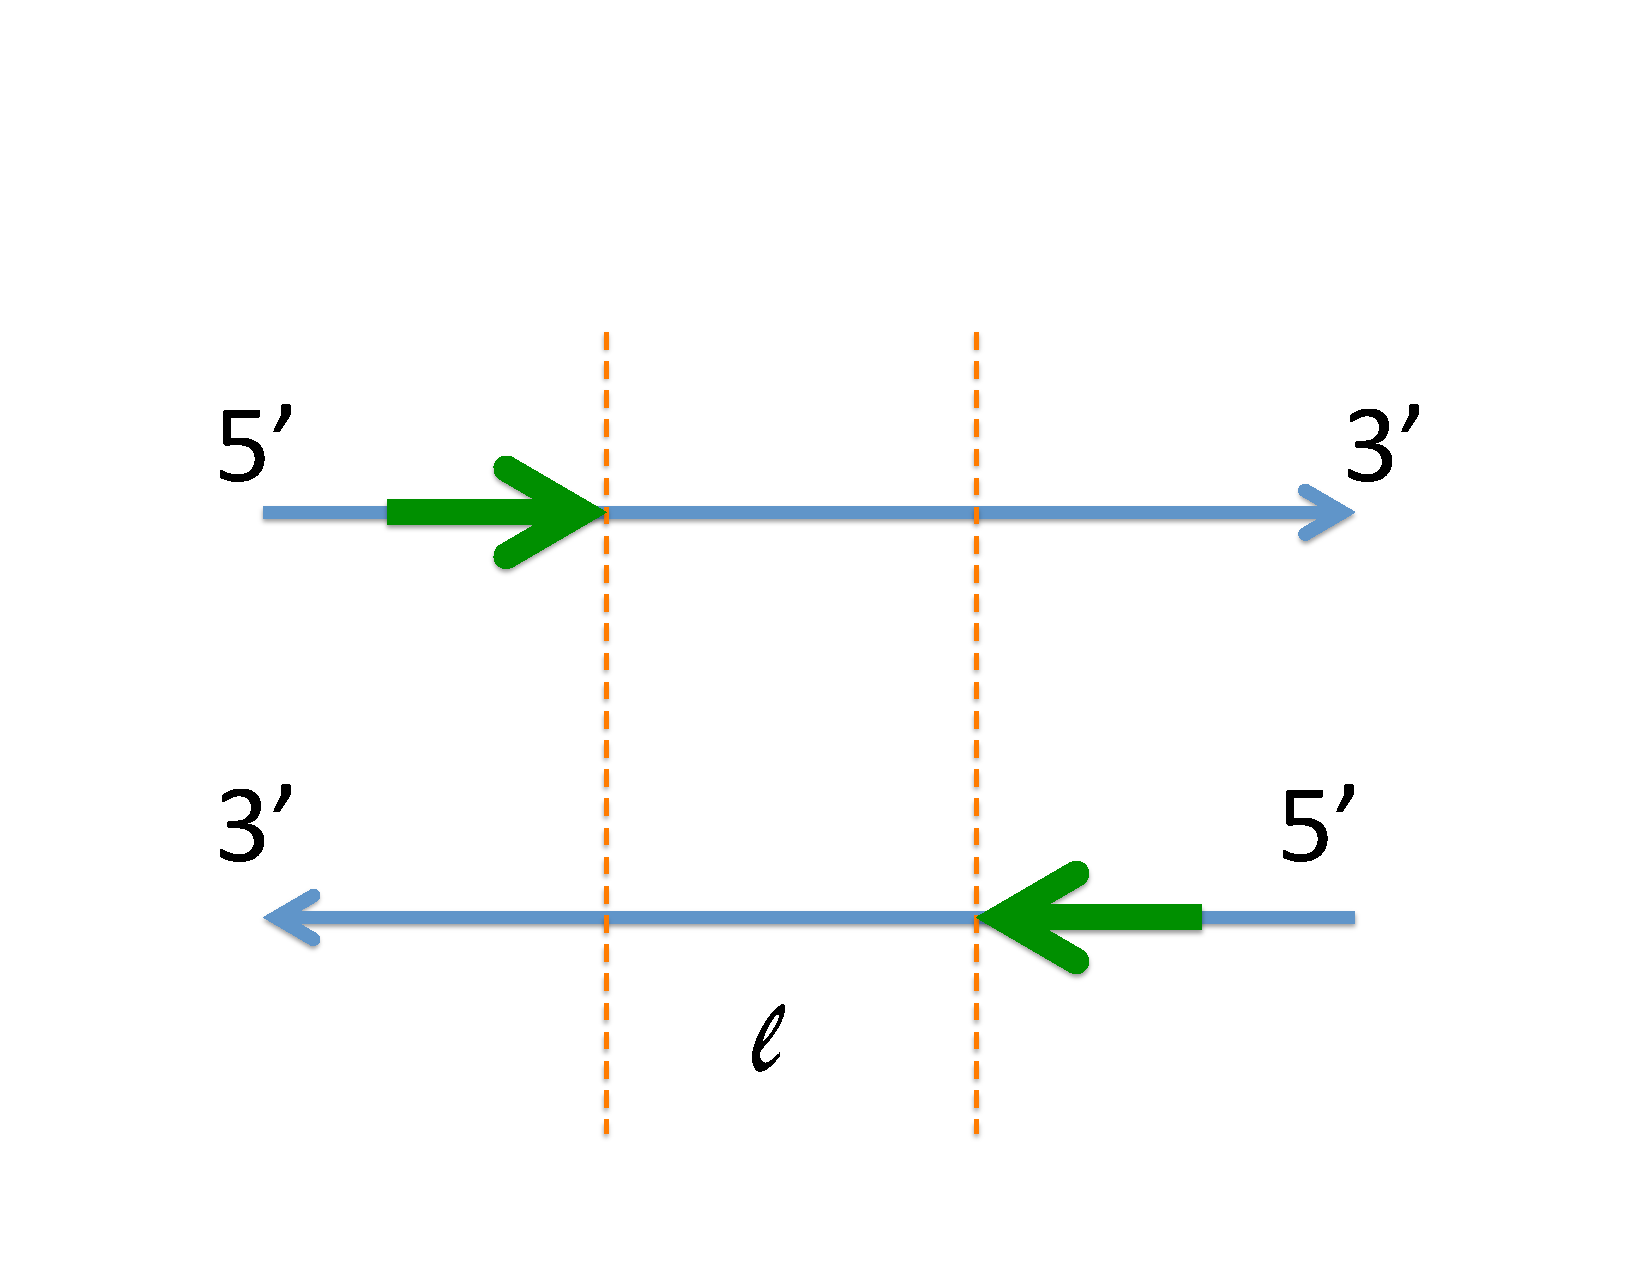
\includegraphics[width=6in]{./bioinformatics/pics/bowtie_example}
\caption{An example of Bowtie, as it tries to align a subsequence in a DNA sequence with another subsequence in another DNA sequence.}
\label{fig:BowtieExample}
\end{figure}

An example of DNA sequences being read by {\tt Bowtie} is shown in Figure \ref{fig:BowtieExample}. \\


Separate the reads into different classes, especially for genomes with lots of single nucleotide polymorphism (SNPS) $\rightarrow$ lots of inversion that need to be sorted.













%%%%%%%%%%%%%%%%%%%%%%%%%%%%%%%%%%%%%%%%%%%%%%
\section{SAM File Format}
\label{sec:SAMFileFormat}

The second field of the {\tt SAM} file format indicates various information about the alignment and pairing. It indicates the call of a proper read, or align read. The majority of the reads don't map well because we are mapping only to the smallest chromosome of the species. The {\it Neurospora crassa} species has 7 chromosomes\dots\ Without paired reads, the numbers are different. \\

Some calculations to determine such information is demonstrated as follows: \vspace{-0.3cm}
\begin{enumerate} \itemsep -4pt
\item 77 = 64 + 8 + 4 + 1
\item 141 = 128 + 8 + 4 + 1
\item 163 = 128 + 32 + 2 + 1. Properly aligned.
\item 83 = 64 + 16 + 2 + 1
\item 99 = 64 + 32 + 2+ 1
\end{enumerate}

Convert {\tt SAM} files to {\tt BAM} files, which are faster to read. {\tt SAM} files are written according to when they (i.e., the subsequences) are found/read; that is, they are written as the subsequences are found. On the other hand, the {\tt BAM} files can be sorted according to their coordinates of the beginning (and, hence, the end) of the subsequences; {\it verify this!!!}. These {\tt BAM} files are sorted from left to right. For control
















